\begin{definition}[Mumford-Shah Functional] % (fold)
\label{def:the_mumford_shah_functional_revisited}

    Let $\Omega \subset \mathbb{R}^{2}$ be a rectangular image domain. In order to approximate an input image $f: \Omega \longrightarrow [0, 1]$ in terms of a piecewise smooth function $u: \Omega \longrightarrow [0, 1]$, Mumford and Shah suggested to minimize the functional
        
        \begin{equation}
            E(u) = \lambda \int_{\Omega} (f - u)^{2} dx + \int_{\Omega \setminus S_{u}} |\nabla u|^{2} dx + \nu \mathcal{H}^{n-1}(S_{u}),
        \label{eq:the_mumford_shah_functional_revisited}
        \end{equation}
    
    where $\lambda, \nu > 0$ are weighting parameters, $S_{u} = S^{n-1}_{u} \cup ... \cup S^{N}_{u}$ and $\mathcal{H}^{1}(S_{u})$ denotes the n-1-dimensional Hausdorff-measure of the curves in $S_{u}$.

\end{definition}
% definition the_mumford_shah_functional (end)

The difference to Chapter 3 is, that we interchanged the set $K = K_{1} \cup ... \cup K_{N}$ to $S_{u} = S^{1}_{u} \cup ... \cup S^{N}_{u}$ and instead of computing $|K|$, the length of the curves, we use the more general notation of measure theory. In the case, where $u \in \Omega \subset \mathbb{R}^{2}$, the n-1-dimensional Hausdorff-measure of $S_{u}$ is nothing but $|S_{u}|$. Another difference to definition \ref{def:the_mumford_shah_functional} is the parameter $\lambda$, which handles the tradeoff between the data fidelity term and the first term in the regularizer. It is swapped and controls now the term where the image $f$ enters the functional. Swapping this parameter does not change the energy at all. So both definitions are totally consistent. As mentioned in the previous chapter, this functional is highly non-convex. The idea to derive a convex saddle-point representation of the Mumford-Shah functional is to make use of some results presented by Alberti, Bouchitte and DalMaso. They applied in (papers...) convex relaxation techniques to approximate the Mumford-Shah Functional by a convex maximization problem. To get this representation, let us first start with introducing some functions.%Then we would be able to apply our primal-dual algorithm.

\section{Convex Relaxation} % (fold)
\label{sec:convex_relaxation}

    %What we are looking for is the (global) minimal value of the piecewise smooth Mumford-Shah functional, i.e. $\min\limits_{u \in X} E(u)$. Another approach would be to minimize the piecewise constant functional where we set the weight $\lambda = \infty$, which we discussed in the last chapter and will not consider for this representation.
    In order to state a convex relaxed model, we need to introduce the characteristic (level set) function.

    \begin{definition}
    \label{def:characteristic_function}
        Let $\Omega \subset \mathbb{R}^{2}$ denote the image plane and let $u \in SBV(\Omega)^{1}$. The upper level sets of $u$ are denoted by the characteristic function $\mathds{1}_{u}: \Omega \times \mathbb{R} \longrightarrow \{ 0, 1 \}$ of the subgraph of $u$:
            \begin{equation}
                \mathds{1}_{u}(x, t) =
                    \left\{
                        \begin{array}{l l}
                            1, & \quad \text{if $t < u(x)$}, \\
                            0, & \quad \text{else}.
                        \end{array}
                    \right.
            \label{eq:characteristic_function}
            \end{equation}
    \end{definition}

    In figure \ref{fig:characteristic_function} one can see an example with a characteristic function in $\mathbb{R}^{2}$ for a function $u \in SBV(\Omega)^{1}$. So, for a one-dimensional signal $u(x)$ the characteristic function becomes a two-dimensional function. It extends the original from with one dimension. In our case, as we consider two-dimensional images, the characteristic function adds another label space and we then act in a cube.

    \begin{figure}[ht]
        \centering
        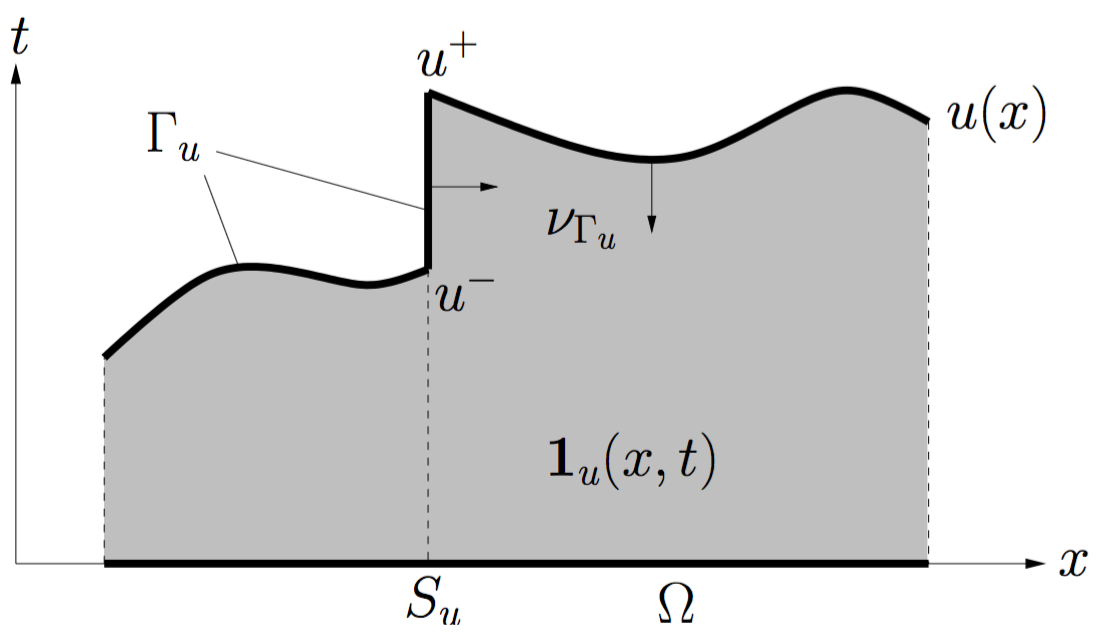
\includegraphics[width=0.7\textwidth]{img/char_func.png}
        \caption[Characteristic Function of a SBV function]{\label{fig:characteristic_function} This picture (taken from \cite{Pock-et-al-iccv09}) shows the characteristic function $\mathds{1}_{u}(x, t)$ of a function $u(x) \in SBV$.}
    \end{figure}

    The gray shaded area is the part where $\mathds{1}_{u}(x, t) = 1$. Otherwise, the characteristic function is set to zero. The upper interface of the gray domain is denoted by $\Gamma_{u}$. This set is the set which holds all parts of the function $u(x)$ and each curve $S_{u}$ which connects the points $u^{-}$ and $u^{+}$. These two points are the last and the first point, respectively, of each partial curve of $u(x)$. Additionally, the notation $\nu_{\Gamma_{u}}$ denotes the normals on $\Gamma_{u}$.

    % \begin{remark}
    %     This lifiting method together with the following theorem assures, that the Mumford-Shah Model we are facing will be convex. As soon as we have a convex optimazation problem we can apply the primal-dual algorithm to solve it.
    % \end{remark}

    Using $\mathds{1}_{u}(x, t)$, one can find in \cite{Alberti-et-al-lnss} and \cite{Alberti-et-al-cvpde} the proposed method of Alberti, Bouchitte and DalMaso along with a proof of this result. We state this theorem in the fashion of \cite{Pock-et-al-iccv09}. We provide it without giving a proof.

    \begin{theorem}[Convex Relaxation of the Mumford-Shah Functional]
    \label{convex_relaxation_of_the_mumford_shah_functional}
        For a function $u \in SBV(\Omega)$ the Mumford Shah functional can be written as
            \begin{equation}
                E(u) = \sup_{\varphi \in K} \int_{\Omega \times \mathbb{R}} \varphi D\mathds{1}_{u}, \label{eq:convex_relaxed_ms}
            \end{equation}
        with a convex set
            \begin{eqnarray}
                K = \bigg\{ \varphi \in C^{0}(\Omega \times \mathbb{R}, \mathbb{R}^{2}) &:& \varphi^{t}(x, t) \ge \frac{\varphi^{x}(x,t)^{2}}{4} - \lambda(t - f(x))^{2}, \\
                &&\bigg| \int^{t_{2}}_{t_{1}} \varphi^{x}(x,s)ds \bigg| \le \nu \bigg\}, \label{eq:set_k_continuous}
            \end{eqnarray}
        where the inequalities in the definition of $K$ hold for all $x \in \Omega$ and for all $t, t_{1}, t_{2} \in \mathbb{R}$.
    \end{theorem}

    \begin{remark}
        \begin{itemize}
            \item We used in the theorem, that we will represent a vector $\varphi \in K \subseteq \mathbb{R}^{n}$ by $\varphi(x, t) = \big( \varphi^{x}, \varphi^{t} \big)^{T}$, where $\varphi(x,t) \in \mathbb{R}^{n}$, $\varphi^{x} \in \mathbb{R}^{n-1}$ and $\varphi^{t} \in \mathbb{R}$.
            \item The idea to approximate the Mumford-Shah Functional is, to maximize the flux of a vector field $\varphi$ through the interface $\Gamma_{u}$. The advantage of this technique is, to get a convex representation of the Mumford-Shah Functional and for this we derive in the following a convex saddle-point formulation. Then we can again make use of the primal-dual algorithm to solve this optimization problem.
        \end{itemize}
    \end{remark}

    Our goal is to minimize \ref{eq:convex_relaxed_ms}. We have
    \begin{equation}
        \min_{u} E(u) = \min_{u} \left( \sup_{\varphi \in K} \int_{\Omega \times \mathbb{R}} \varphi D\mathds{1}_{u} \right)
        \label{eq:minimize_convex_relaxed_ms}
    \end{equation}

    To compute the minimizer of this formulation we first need to substitute $\mathds{1}_{u}$ by a generic function
        \begin{equation}
            v(x, t): \Omega \times \mathbb{R} \longrightarrow [0, 1] \,\, \textnormal{and} \,\, \lim_{t \rightarrow -\infty} v(x, t) = 1, \, \, \, \lim_{t \rightarrow +\infty} v(x, t) = 0.
        \label{eq:generic_functions}
        \end{equation}

    % This substitution takes into account that the image $f$ and its approximation $u$ map into $[0, 1]$. For binary images changing $\mathds{1}_{u}$ to $v$ would not be necessary. Unfortunatelly, this substitution of the functions makes the proposed method inexact. It still computes a lower bound to the global, optimal solution, but it only converges to the exact solution if $f$ is binary. For more information we refer to \cite{Pock-et-al-iccv09}. 
    Overall, we are going to face the following convex optimization problem:
        \begin{equation}
            \min_{v \in [0, 1]} \sup_{\varphi \in K} \langle v, D\varphi \rangle = \min_{v \in [0, 1]} \sup_{\varphi \in K} \int_{\Omega \times \mathbb{R}} \varphi Dv.
            \label{eq:continous_saddle_point_problem}
        \end{equation}

    According to \cite{Pock-et-al-iccv09} there is no proof, that finding an optimal pair $(v^{\ast}, \varphi^{\ast})$ for the optimization problem \ref{eq:continous_saddle_point_problem} leads to the global minimizer of equation \ref{eq:the_mumford_shah_functional_revisited}. Further, they state that only if $v^{\ast}$ is binary one gets indeed the global minimum of the Mumford-Shah Functional.

    In the next section we will consider this optimization problem \ref{eq:continous_saddle_point_problem} in the discrete version. Additionally, we propose the corresponding operators and compute the proximity operators - which then will be euclidean projections.

% section convex_relaxation (end)